
\section{Synthesizing Optimizations}

For every cut extracted from an LLVM function, \minotaur{}'s goal is to
find a cheaper way to compute the value returned by that cut.


\subsection{Enumeration of Partial Symbolic Candidates}

\begin{table}[t]
  \centering
  \begin{tabular}{ r | l }
    \hline
    \textbf{Operation Type} & \textbf{Instructions} \\
    \hline \hline
    Unary integer ops & ctpop, ctlz, cttz, bitreverse, bswap \\
    Unary floating point ops & fneg, fabs, fceil, ffloor, frint, \dots \\
    Binary integer ops & add, sub, mul, udiv, sdiv, umax, umin, smax, smin\\
    Binary floating point ops & fadd, fsub, fmul, fdiv, frem, \dots \\
    Bitwise ops & and, or, xor, shl, lshr, ashr \\
    Data movement ops & extractelement, insertelement, shufflevector \\
    Comparisons & icmp, fcmp, select \\
    Conversions & zext, sext, trunc, fptrunc, fpext, fptosi, sitofp, fptoui, uitofp \\
    Intrinsic functions & 165 vector intrinsics \\
    \hline
  \end{tabular}
  \caption{List of operations generated by Minotaur}
  \label{tab:operations}
\end{table}


\minotaur{} creates \emph{partially symbolic} candidates where
instructions are represented concretely, but constants are symbolic.
%
Symbolic constants reduce the size of the search space without giving
up synthesis power.


\minotaur{} generates every candidate that fits into a configurable bound
on the number of new instructions to synthesize.
%
However, LLVM's \texttt{bitcast} instruction, which changes the type
of an SSA value without changing its representation, does not count
towards this limit.
%
This is because \minotaur{} takes a low-level, untyped view of values.
%
For example, it internally treats a 16-way vector of 8-bit values the
same as an 8-way vector of 16-bit values: both of these are simply
128-bit quantities.
%
This lack of type enforcement allows \minotaur{} to find interesting,
low-level optimizations such as those that use bitwise operations to
rapidly perform certain floating point operations.
%
(Example 5 in Section~\ref{sec:examples} shows one of these.)


\minotaur{}'s enumeration algorithm generates a wide variety of instructions,
including arithmetic, bitwise, data movement, comparisons, conversions,
and calls to intrinsic instructions.
%
Table~\ref{tab:operations} shows the list of operations that are
supported by \minotaur{}'s synthesis algorithm.



\subsection{Checking Refinement}


\begin {figure}[tbp]
  \centering
  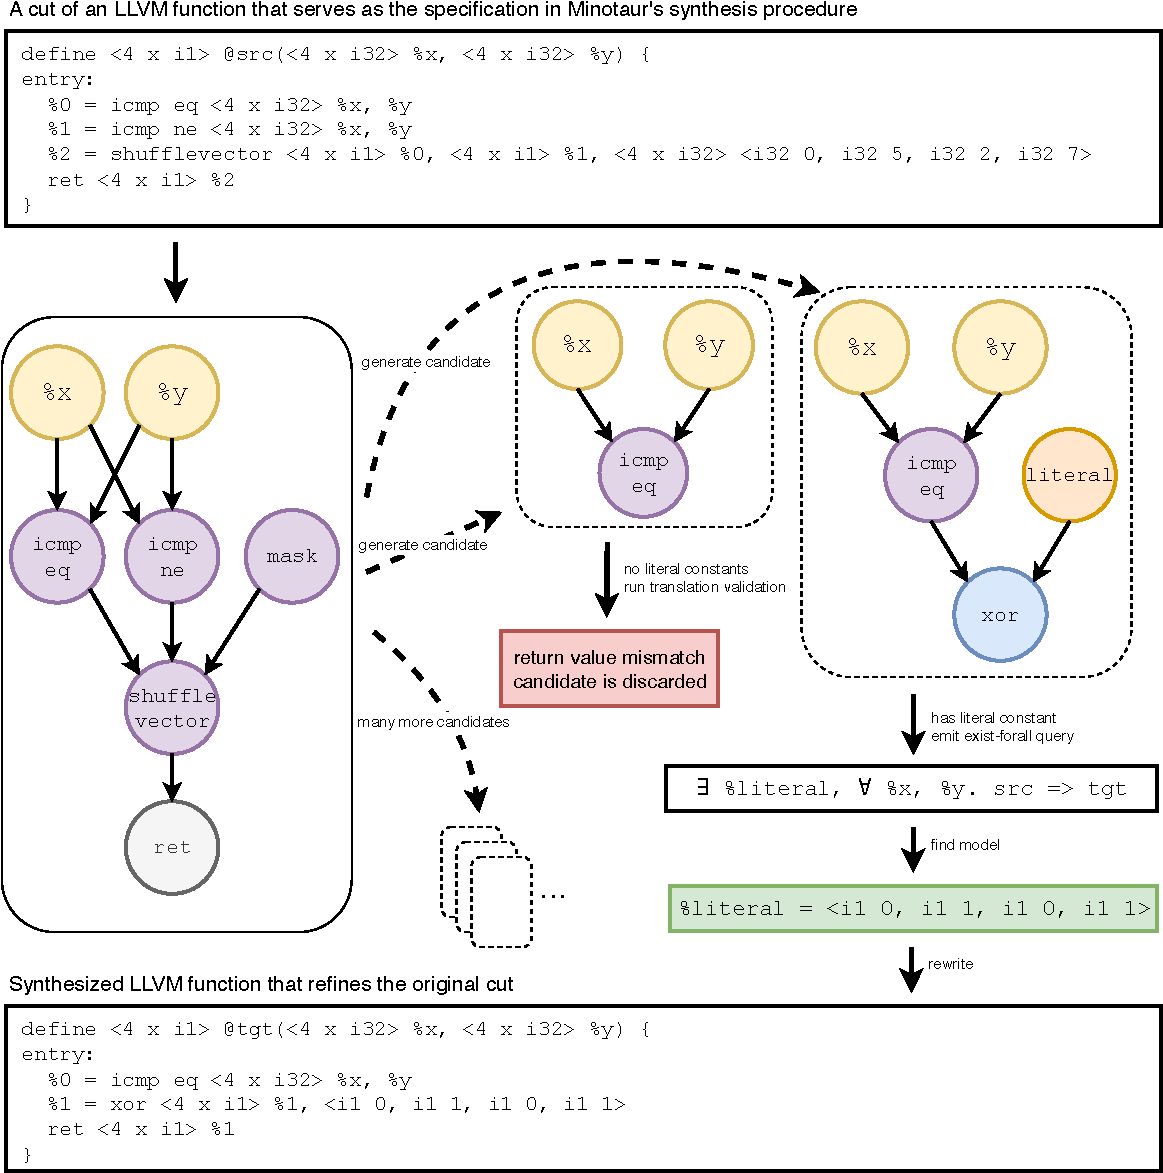
\includegraphics[width=\linewidth]{figures/solve_literal.pdf}
  \caption{Example of synthesizing a rewrite that contains literal
    constants.  Purple nodes are instructions reused from the original
    cut; blue and orange nodes are synthesized instructions and
    literal constants.}
  \label{fig:synthesizing}
\end{figure}

\minotaur{} uses Alive2 to eliminate every candidate that does not refine
the specification.
%
Figure~\ref{fig:synthesizing} illustrates this process.
%
For the incoming cut shown in the top of the figure, \minotaur{}
enumerates possible rewrites that could be applied to the cut.
%
For a candidate that has literal constants, \minotaur{} will ask Alive2 to
emit a exists-forall query to find a model for the literal constants
such that the rewrite refines the cut forall the inputs.
%
If the query is satisfiable, \minotaur{} will apply the rewrite to the
cut.


\subsection{Identifying Profitable Rewrites}

Predicting throughput of code running on modern microprocessors is not
straightforward.
%
To help developers improve performance-critical code, the LLVM Machine
Code Analyzer (LLVM-MCA)~\cite{llvmmca} was created.
%
It is an interactive tool that emits a graphical depiction of pipeline
behavior, but its functionality can also be accessed programmatically,
and this is what \minotaur{} does.


We estimate the cost of a rewrite in two places.
%
First, after enumerating candidates but before performing refinement
checks, we sort them in order of increasing cost using LLVM's
TargetTransformInfo~\cite{tti}; a cost model that roughly captures
execution cost on the target, and is cheap to compute.
%
We do this to ensure that likely-beneficial rewrites are tested first,
since we often run \minotaur{} under a timeout for each optimization site.
%
Second, rewrites that have been confirmed to be refinements of the
original code are compiled to x86-64 object code and then analyzed
LLVM-MCA~\cite{llvmmca}, the machine code analyzer.
%
This cost model is more accurate but considerably slower than the
first one.
%
\minotaur{} only applies a rewrite if its estimated cost, using LLVM-MCA,
is lower than that of the original cut.


Although LLVM-MCA can estimate the cycle cost of LLVM functions, we instead use
the number of uOps (``micro-operations,'' a modern x86 processor's internal
instruction set) as the estimated cost.
%
This choice was driven by empirical data: after extensive
experimentation, we determined that, for our purposes, uOps are a
better performance predictor than cycles.



\subsection{Representing and Caching Rewrites}
\label{sec:rewrite}

\minotaur{} stores each potential rewrite as a pair: $(C, S)$
where $C$ is a cut, represented by a function in LLVM
Intermediate Representation (IR), and $S$ is a rewrite description---an
expression in \minotaur's own intermediate representation that describes a
different way to compute the return value of $C$.
%
Rewrite descriptions are directed acyclic graphs containing nodes that represent
operations, and edges representing data flow.
%
Although the elements found in \minotaur{} IR are similar to those found
in LLVM IR, we could not reuse LLVM IR to represent rewrites since
LLVM IR does not support incomplete code fragments, and also rewrites
must contain enough information to support connecting the new code in
the rewrite to code in the unoptimized function.


To support caching, rewrites must be serializable.
%
The cut $C$ can be serialized using existing LLVM functionality, and we
created a simple S-expression syntax for serializing the $S$ part.
%
Figure~\ref{fig:syntax} shows the syntax of the IR\@.
%
For example, if the returning value of $C$, a 32-bit instruction is
replaced by left shift by one bit position, the textual format for
the expression is \texttt{(shl (val i32 \%0), (const i32 1), i32)}.


Rewrites are cached in a Redis instance: this implementation choice
allows the cache to be persistent across multiple \minotaur{} runs and
also makes the cache network-accessible.
%
Synthesis can be done online---during compilation---but also
offline, in a mode where \minotaur{} extracts cuts into the Redis
cache but does not perform synthesis.
%
In this mode, compilation is only slowed down by a few percent.
%
\minotaur's offline mode is designed for batch processing.
%
In this mode, a separate program called \texttt{cache-infer} retrieves
cuts from the cache, runs synthesis on them, and stores any
optimizations that it discovers back into the cache.
%
Unlike the online mode, which runs synthesis tasks one after the
other, offline mode can run all synthesis jobs in parallel.



\begin{figure}[tbp]
  \begin{tabular}{r c l}
    \emph{Op} &::=& \emph{Inst} $\vert$ \emph{Constant} $\vert$ \emph{Value} \\
    \emph{Inst}  &::=& (\emph{UnaryOp} \emph{Op}, \emph{Type}) $\vert$ (\emph{BinaryOp} \emph{Op}, \emph{Op}, \emph{Type}) $\vert$ (\emph{Conversion} \emph{Op}, \emph{Type}) $\vert$\\
              && (insertelement \emph{Op}, \emph{Op}, \emph{Op}) $\vert$ (extractelement \emph{Op}, \emph{Op})  $\vert$\\
              && (\emph{Comparison} \emph{Op} \emph{Op}) $\vert$ (select \emph{Op}, \emph{Op}, \emph{Op}) $\vert$ (\emph{Intrinsic} \emph{Op}, \emph{Op}) $\vert$ \\
              && (shufflevector \emph{Op}, \emph{Op}, \emph{Constant}) \\
    \emph{Constant} &::=& (const \emph{Type} \texttt{number-literal}) \\
    \emph{Value} &::=& (val \emph{Type} \texttt{llvm-identifier}) \\

    \emph{Type} &::=& \emph{ScalarType} $\vert$ <elements $\times$ \emph{ScalarType}> \\
    \emph{ScalarType} &::=& i1 $\vert$ i8 $\vert$ i16 $\vert$ i32 $\vert$ i64 $\vert$ half $\vert$ float $\vert$ double $\vert$ fp128 \\
    \emph{BinaryOp} &::=& xor $\vert$ and $\vert$ or $\vert$ add $\vert$ sub $\vert$ mul $\vert$ udiv $\vert$ sdiv $\vert$ \\
                && ashr $\vert$ lshr $\vert$ shl $\vert$ umax $\vert$ umin $\vert$ smax $\vert$ smin\\
                && fadd $\vert$ fsub $\vert$ fmul $\vert$ fdiv $\vert$ copysign $\vert$ \\
                && fmaximum $\vert$ fminimum $\vert$ fmaxnum $\vert$ fminnum \\
    \emph{UnaryOp} &::=& ctpop $\vert$ ctlz $\vert$ cttz $\vert$ bswap $\vert$ bitreverse $\vert$\\
                      && fneg $\vert$ fabs $\vert$ fceil $\vert$ ffloor $\vert$ frint $\vert$ fround $\vert$ ftrunc $\vert$ fnearbyint $\vert$ froundeven \\
    \emph{Conversion} &::=& zext $\vert$ sext $\vert$ trunc $\vert$\\
                    && fptrunc $\vert$ fpext $\vert$ fptosi $\vert$ sitofp $\vert$ fptoui $\vert$ uitofp \\
    \emph{Comparison} &::=& eq $\vert$ ne $\vert$ ult $\vert$ ule $\vert$ slt $\vert$ sle $\vert$\\
                && oeq $\vert$ ogt $\vert$ oge $\vert$ olt $\vert$ ole $\vert$ one $\vert$ ord $\vert$ ueq $\vert$ ugt $\vert$ uge $\vert$ ult $\vert$ ule $\vert$ une $\vert$ uno \\
    \emph{Intrinsic} &::=& ssse3.phadd.d.128 $\vert$ avx2.pavg.b  $\vert$ \dots (165 intrinsics in total) \\
  \end{tabular}
  \caption{Syntax for Minotaur rewrites}
  \label{fig:syntax}
  % \Description[syntax]{Minotaur syntax}
\end{figure}



\subsection{Integration with LLVM}

\minotaur{} is loaded into LLVM as a shared library where it runs as an
optimization pass.
%
We arranged for it to run at the end of LLVM's auto-vectorization pipeline.
%
We call the Dead Code Elimination pass after Minotaur to
clean up the code.
